\chapter{Overview of \acrshort{athlet} and \acrshort{nut} software}\label{chapter:athlet-nut}

\section{\acrshort{athlet}}
\label{sec:athlet-overview}


%The thermal-hydraulic system code \acrfull{athlet} code is developed by \acrshort{grs} for the analysis of the whole spectrum of operational conditions, incidental transients, design-basis accidents and beyond design-basis accidents without core damage anticipated for nuclear energy facilities \cite{grs:athlet-info}. The code provides specific models and methods for the simulation of many types of nuclear power plants comprising current light water reactors (PWR\footnote{Pressurized Water Reactor}, BWR\footnote{Boiling Water Reactor}, WWER\footnote{Water-Water Energetic Reactor}, HPCR\footnote{High Power Channel-type Reactor}), advanced Generation III+ and IV reactors as well as SMRs\footnote{Small Modular Reactor} \cite{grs:athlet-info}.\\


\acrfull{athlet} software is developed by \acrshort{grs} for an analysis of the whole spectrum of operational conditions, incidental transients, design-basis accidents and beyond design-basis accidents without core damage anticipated for nuclear energy facilities \cite{grs:athlet-info}. The code provides specific models and methods to simulate many types of nuclear power plants, comprising current light water reactors (PWR\footnote{Pressurized Water Reactor}, BWR\footnote{Boiling Water Reactor}, WWER\footnote{Water-Water Energetic Reactor}, HPCR\footnote{High Power Channel-type Reactor}), advanced Generation III+ and IV reactors as well as SMRs\footnote{Small Modular Reactor} \cite{grs:athlet-info}.\\



Physical processes inside of hydraulic circuits of light water reactors can be naturally described by a two-phase thermo-fluiddynamic model based on equations of conservation mass, momentum and energy for liquid and vapor phases i.e. Equations \ref{eq:athlet-1} - \ref{eq:athlet-7}, \cite{lt:ATHLMaM}.\\

1. Liquid mass
\begin{equation} \label{eq:athlet-1}
\frac{\partial ((1-\alpha)\rho_{l})}{\partial t} + \nabla ((1-\alpha) \rho_{l} \vec{w_{l}}) = - \psi
\end{equation}


2. Vapor mass
\begin{equation} \label{eq:athlet-2}
\frac{\partial (\alpha \rho_{v})}{\partial t} + \nabla (\alpha \rho_{v} \vec{w_{v}}) = \psi
\end{equation}


3. Liquid momentum
\begin{equation} \label{eq:athlet-3}
\frac{\partial ((1-\alpha) \rho_{l} \vec{w_{l}})}{\partial t} + \nabla ((1-\alpha) \rho_{l} \vec{w_{l}} \vec{w_{l}}) + \nabla ((1 - \alpha)p) = \vec{F_{l}}
\end{equation}


4. Vapor momentum
\begin{equation} \label{eq:athlet-4}
\frac{\partial (\alpha \rho_{v} \vec{w_{v}})}{\partial t} + \nabla (\alpha \rho_{v} \vec{w_{v}} \vec{w_{v}}) + \nabla (\alpha p) = \vec{F_{v}}
\end{equation}


5. Liquid energy
\begin{equation} \label{eq:athlet-5}
\frac{\partial \Big[ (1-\alpha)\rho_{l}(h_{l} + \frac{1}{2} \vec{w_{l}} \vec{w_{l}} - \frac{p}{\rho_{l}}) \Big]}{\partial t} + \nabla \Big[ (1-\alpha)\rho_{l}\vec{w_{l}}(h_{l} + \frac{1}{2} \vec{w_{l}} \vec{w_{l}}) \Big] = - p \frac{\partial (1 - \alpha)}{\partial t} + E_{l}
\end{equation}


6. Vapor energy
\begin{equation} \label{eq:athlet-6}
\frac{\partial \Big[ \alpha \rho_{v}(h_{v} + \frac{1}{2} \vec{w_{v}} \vec{w_{v}} - \frac{p}{\rho_{v}}) \Big]}{\partial t} + \nabla \Big[ \alpha\rho_{v}\vec{w_{v}}(h_{v} + \frac{1}{2} \vec{w_{v}} \vec{w_{v}}) \Big] = - p \frac{\partial \alpha}{\partial t} + E_{v}
\end{equation}

7. Volume vapor fraction
\begin{equation} \label{eq:athlet-7}
	\alpha = \frac{V_{v}}{V}
\end{equation}


The notation is as follows: $p$ - pressure of a liquid-vapor mixture, $\psi$ - a mass source term, $\vec{F}$ - an external composite force acting on a CV\footnote{CV - Control Volume}, $E$ - an external composite energy source term within a CV, subscripts $l$ and $v$ denote liquid and vapor phases, respectively. \\


% Finite volume and 1D discritiazation 
Spacial integration of the conservation equations, System \ref{eq:athlet-1} - \ref{eq:athlet-7}, is performed on basis of the finite volume method using one-dimensional problem formulation, Figure \ref{fig:introduction-1d-fvm}. Then, the system is transformed to an initial value problem of a system of non-autonomous \acrlong{ode}s (\acrshort{ode}s) by means of certain additional mathematical transformations, see \cite{lt:ATHLMaM}.\\


\figpointer{\ref{fig:introduction-1d-fvm}}
\begin{figure}[htpb]
  \centering
  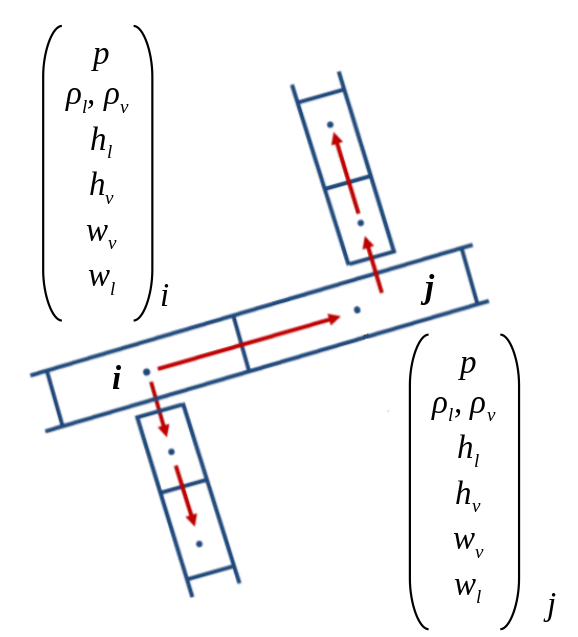
\includegraphics[width=0.5\textwidth]{figures/introduction-1d-fvm.png}
\caption[One-dimensional finite volume formulation of a thermo-hydraulic problem in \acrshort{athlet}]{One-dimensional finite volume formulation of a thermo-hydraulic problem in \acrshort{athlet}, \cite{tims-presentation}, where $T_l$ - a temperature of liquid inside of a CV; $T_v$ - a temperature of vapor inside a CV; $X_m$ - mass quality; $G$ - mass flow of a liquid-vapor mixture; $W$ - a velocity component of a liquid-vapor mixture perpendicular to a CV boundary; $A_l$ - an area occupied by the liquid fraction on a CV boundary, $A_l$ - an area occupied by the vapor fraction on a CV boundary; $Q$ - an external heat transfer}
\label{fig:introduction-1d-fvm}
\end{figure}


%Finally, the system is transformed to a non-autonomous system of \acrlong{ode}s (\acrshort{ode}s) and expressed as an initial value problem, equation \ref{eq:athlet-8}, after spatial finite volume integration and many mathematical transformations \cite{lt:ATHLMaM}. 


\begin{equation} \label{eq:athlet-8}
	\frac{dy}{dt} = f(t,y), \;  t_{0} \leq t \leq t_{F} \; y(t_{0}) = y_{0}
\end{equation}

where $y \in \mathbb{R}^{n}$ is a composite vector of variables, $f$ is a non-linear function such that $f : \mathbb{R} \times \mathbb{R}^{n} \supset \Omega  \rightarrow \mathbb{R}^{n}$  .\\


%\cite{lt:ATHLMaM}
% Rosenbrock-Wanner
%According to \citetitle{lt:ATHLMaM} \cite{lt:ATHLMaM}, System \ref{eq:athlet-8} is stiff and thus must to be solved with an implicit solver. Rosenbrock methods belong to a class of linearly implicit ones which are capable of solving such stiff systems of \acrshort{ode}s efficiently. The methods replace non-linear systems with a sequence of linear ones, however, some stability and accuracy properties are usually lost \cite{blom2013rosenbrock}. An additional drawback of the methods is a computation of the exact Jacobian at every time step which affects the overall computational cost.\\

According to \citetitle{lt:ATHLMaM} \cite{lt:ATHLMaM}, System \ref{eq:athlet-8} is stiff and thus must to be solved with an implicit solver. To avoid a high computational cost of a fully implicit method, \acrshort{athlet} makes use of an extrapolation ansatz based on the linearly implicit Euler method. This may be interpreted as a six stage W-method where the exact Jacobian information is not required. However, fresh information of the Jacobian matrix during a numerical simulation greatly improves stability and robustness of the method. Therefore, several mechanisms have been implemented in \acrshort{athlet} to closely monitor and, if it is required, to update a Jacobian matrix approximation using the finite difference method.\\


%To decrease the cost and preserve sufficient accuracy of numerical integration, \acrshort{athlet}, instead, uses a W-method of the third order. W-methods belong to the family of Rosenbrock methods, however, calculate the Jacobian matrix occasionally. The \acrshort{athlet} developers spent much of their time and efforts to develop heuristics to identify instances of time when a next evaluation of the Jacobian must be performed. In other words, the algorithm can re-use the same Jacobian matrix approximation between steps with some partial matrix updates. However, when a hydraulic circuit state drastically changes due to transitivity, the evaluation of the full Jacobian is demanded.\\


\figpointer{\ref{fig:introduction-w-method-scheme}}
\begin{figure}[htpb]
  \centering
  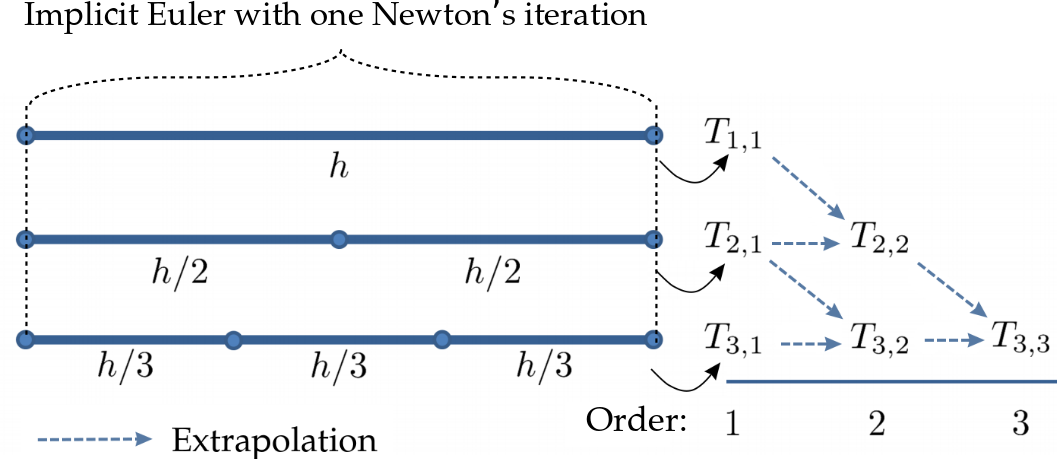
\includegraphics[width=0.8\textwidth]{figures/introduction-rosenbrock-scheme.png}
\caption[A general view on the 6-stage W-method implemented in \acrshort{athlet}]{A general view on the 6-stage W-method implemented in \acrshort{athlet} (based on \cite{tims-presentation}), where $T_{1,1} = y_{0} + y_{1,0}$; $T_{2,1} = y_{0} + y_{2,0} + y_{2,1}$; $T_{3,1} = y_{0} + y_{3,0} + y_{3,1} + y_{3,2}$ 
}

\label{fig:introduction-w-method-scheme}
\end{figure}

In the general case, a step of the W-method method, implemented in \acrshort{athlet}, can be viewed as a sequence of six stages in the following way. Each stage uses the implicit Euler method and exactly one Newton's iteration to evaluate values of vector $y$ at the next integration step $h$ with different accuracy. Then, the obtained values are extrapolated, in order shown in Figure \ref{fig:introduction-w-method-scheme}, to achieve the third order of numerical integration. By and large, the algorithm can be expressed in a compact form of Equation \ref{eq:athlet-9}.

%\begin{equation} \label{eq:athlet-9}
%	((h \gamma)^{-1}I - J) \Delta z^{l}_{i} = - h^{-1} z^{l}_{i} + f(t_0 + \tau_{i} h, y_{0} + z^{l}_{i})
%\end{equation}

 \begin{equation} \label{eq:athlet-9}
        (I - h_{i}J)\delta y_{ij} = h_{i} f(t_{0} + j \cdot h_{i}, y_{0} + \sum^{j-1}_{l = 0} \delta y_{il}) + h^{2} \frac{\partial f_{0}}{\partial t}
    \end{equation}

where $J \approx \frac{\partial f}{\partial y}$ - an approximation of Jacobian matrix; $i = 1, 2, 3$; $j=0, \dots, i - 1$; $h_{i} = h / i$.

%where $\Delta z^{l}_{i} = z^{l+1}_{i} - z^{l}_{i}$; $z^{l}_{i} = y^{l}_{i} - y^{l}_{i - 1}$; $J \approx \frac{\partial f}{\partial y}$ - approximation of Jacobian matrix; $l = 1,2$ - Newton's iteration index; $i = 1, 2, 3$ - integration step index.\\


\section{\acrshort{nut}}

\acrfull{nut} can be viewed as a container of various dense and sparse linear algebra subroutines which can run in parallel on distributed-memory machines. \acrshort{nut} design follows a paradigm of the \textit{Adapter/Wrapper} pattern which provides a uniform common interface for its services to any application that follows a certain communication protocol. Currently, only \acrshort{athlet} can communicate with \acrshort{nut}. However, more \acrshort{grs} applications are going to adopt the protocol in the future and will be able to operate with \acrshort{nut} as well. The approach, implemented in \acrshort{nut}, helps to achieve re-usability, flexibility and extensibility properties of the code.\\


Currently, \acrshort{nut} is based heavily on \acrfull{petsc}. It is one of the most widely used parallel numerical software  libraries \cite{wiki:petsc-general-info}. It includes a large suite of parallel linear and nonlinear equation solvers as well as a software-infrastructure to handle computations on distributed-memory machines by means of  \acrfull{mpi} and specific data structures. Fortunately, through a careful selection of the design pattern, \acrshort{nut} can be easily extended to provide an extra service or an external library access which has not been implemented in \acrshort{petsc} yet.\\ 


\section{\acrshort{athlet}-\acrshort{nut} coupling}
\label{sec:athlet-nut-coupling}

\figpointer{\ref{fig:introduction-nut-process-groups}}
\begin{figure}[htpb]
  \centering
  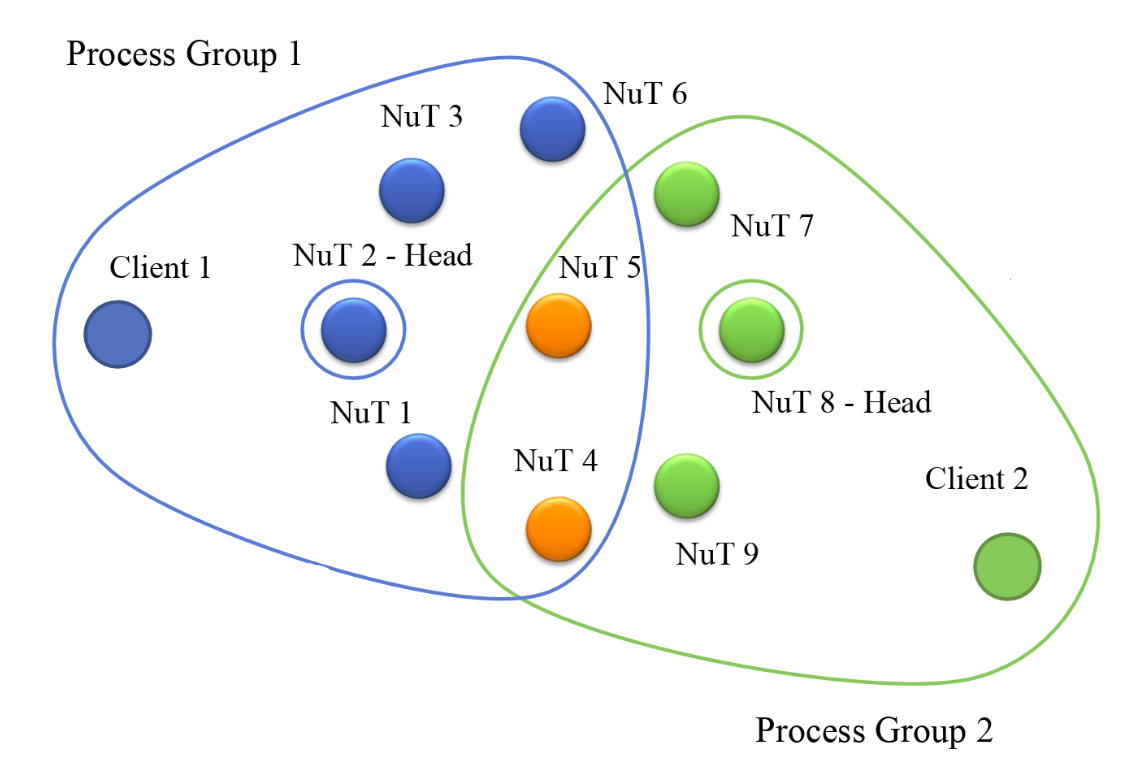
\includegraphics[width=0.8\textwidth]{figures/introduction-nut-process-groups.png}
\caption{An example of \acrshort{nut} process groups}
\label{fig:introduction-nut-process-groups}
\end{figure}

Coupling of \acrshort{nut} with \acrshort{grs} tools is based on the client-server architecture where \acrshort{nut} acts as a server and the tools can be viewed as clients. Communication between two parts is done via \acrshort{mpi}.\\


To provide a clear and concise external interface, \acrshort{nut} contains a client module called "\acrshort{nut} Plug-in". It can be  considered as a socket, from the client side by analogy with the Transmission Control Protocol (TCP). The plug-in hides all \acrshort{mpi} calls to the sever which considerably improves readability of the code.\\


% communicators
In principle, \acrshort{nut} allows multiple clients to work concurrently with the server. To handle communication traffic, \acrshort{nut} splits the default \acrshort{mpi} communicator at start-up time of the application into appropriate process groups, as it is shown in Figure \ref{fig:introduction-nut-process-groups}.\\



The design of \acrshort{nut} allows sharing of some \acrshort{nut}-\acrshort{mpi} processes among different process groups due to performance reasons i.e. a finite number of processing units on hardware. To resolve possible deadlocks, each process group has its own representative, called the head. Each client has two views on its respective group which is achieved by means of distinct \acrshort{mpi} communicators. The first communicator is responsible for client-head communication whereas the second one allows the client to talk to any \acrshort{nut} process within the group.\\



A general view of client-server communication looks like a 3-way handshake in the following way: a client sends a request to the head which is a signal to reserve all compute-units of the group for an upcoming task. Having possessed the resources and prepared them for a specific service, the head notifies the client about a resource acquisition and the entire process group waits for data. Afterwards, the client sends data either to a specific \acrshort{nut}-process or to the entire group using the second communicator and waits for a result of the service. According to the current implementation of \acrshort{nut}, the communication between a client and server is synchronous i.e. a client gets blocked while waiting for a result from the server. \\


A general view on \acrshort{athlet}-\acrshort{nut} software coupling is given in Figure \ref{fig:introduction-athlet-nut-coupling} where  \acrshort{athlet} is responsible for marching the numerical time-integration process whereas \acrshort{nut} computes solutions of linear systems derived from Equation \ref{eq:athlet-9}.\\


%As an example, Figure \ref{fig:introduction-athlet-nut-coupling} represents a general view of \acrshort{athlet}-\acrshort{nut} coupling where \acrshort{athlet} is responsible for marching of the numerical integration solver whereas \acrshort{nut} computes solutions of Systems \ref{eq:athlet-9}.\\


\figpointer{\ref{fig:introduction-athlet-nut-coupling}}
\begin{figure}
  \centering
  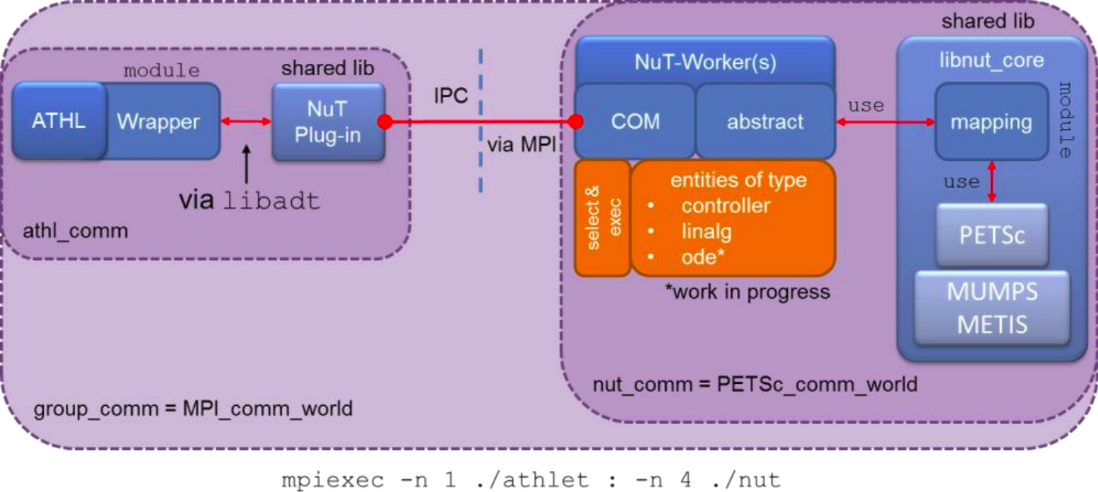
\includegraphics[width=0.75\textwidth]{figures/introduction-athlet-nut-coupling.png}
    \caption{\acrshort{athlet}-\acrshort{nut} software coupling}
\label{fig:introduction-athlet-nut-coupling}
\end{figure}


Partial and full Jacobian matrix updates derived from finite differences are computed on the client side since only a client has access to the function $f$ of Equation \ref{eq:athlet-8}. Due to transformations of the underlying system of \acrlong{pde}s (\acrshort{pde}s) and specifics of finite volume discretization, the Jacobian matrix is sparse and, therefore, \acrshort{athlet} uses a matrix compression algorithm  described in Section \ref{sec:jacobian-matrix-compression} to reduce an amount of Jacobian column evaluations. Having computed a matrix column, \acrshort{athlet} immediately broadcasts it to its entire \acrshort{nut} process group by means of the 3-way handshake mechanism described above. It is worth mentioning that this approach allows to circumvent potential memory limits on the client side and thus store the entire sparse Jacobian matrix in a distributed fashion on the server. In other words, \acrshort{athlet} never holds the entire Jacobian matrix in its memory; conversely, the matrix is distributed across multiple \acrshort{nut} processes according to the block-row distribution scheme induced by \acrshort{petsc}. In turn, \acrshort{nut} is waiting for the entire Jacobian matrix information from \acrshort{athlet} and starts solving Systems \ref{eq:athlet-9} right after receiving the corresponding request from the client.\\


